This work makes available the very first dataset containing ground truth memorability of constituent objects from a highly diverse image set. In this section, we show that our dataset can be used to benchmark computational memorability models and serve as a stepping stone in the direction of automated object memorability prediction.

\vspace{3pt}\noindent\textbf{Baseline models:} As a first step, we propose a simple baseline model that utilizes a conv-net \cite{krizhevsky12,jia14} trained on the ImageNet dataset \cite{deng09}. Since object categories play an important role in determining object memorability (Section \ref{sec:obLabel}), and deep learning models have recently been shown to achieve state-of-the-art results in various recognition tasks, including object recognition \cite{cnn14,lee2009convolutional}, we believe  that this simple model can serve as an adequate baseline for object memorability prediction. We first generated object proposals by using MCG, a generic object proposal method proposed in \cite{arbelaez14}. Next, we trained a support vector regressor (SVR) using $6$-fold cross-validation on the original segments to map deep features to memorability scores. We used this model to predict memorability scores for the top $K=20$ segments in each image, after the image segments are ranked using MCG. After  predicting these memorability scores, memorability maps were generated by averaging the scores of the top $K$ segments at the pixel level. Since image features like SIFT \cite{lowe04} and HOG \cite{dalal05} have previously been shown to achieve good performance in predicting image memorability \cite{isola11,isola14}, we built a second baseline model using these features for comparison. Training and testing of this model was performed similar to the conv-net model.

\vspace{3pt}\noindent \textbf{Evaluation: } To evaluate the accuracy of the predicted object memorability maps, we computed the rank correlation between the mean predicted memorability score inside each of the object segments and their ground truth memorability scores. These results are reported in Figure \ref{fig:benchmark}. Clearly, the conv-net baseline, DL-MCG, performs considerably well ($\rho = 0.39$). In contrast, the baseline trained using HOG and SIFT, H+S, achieves a much lower performance ($\rho = 0.27$). Saliency maps generated from saliency algorithms are also likely to have some degree of overlap with memorability and are therefore worth comparing to our baseline, especially given the absence of other memorability prediction methods\footnote{The only other algorithm that generates memorability maps was proposed in \cite{khosla12}. We contacted the authors and they said they will be releasing an updated version of their paper and codes soon. We will add it to the comparison once they release the code.}. To this end, we included $8$ state-of-the-art saliency methods (top performing methods according to benchmarks in \cite{borji13,borji12}): GB \cite{gb}, AIM \cite{aim}, DV \cite{dv}, IT \cite{it}, GC \cite{gc}, PC \cite{pc}, SF \cite{sf}, and FT \cite{ft} to our comparison. Figure \ref{fig:benchmark}) shows that the H+S baseline is outperformed by most saliency methods. Thus, even though models using SIFT and HOG have previously demonstrated high predictive power for image memorability, they may not be as well suited for the task of predicting object memorability. The deep-net baseline model, DL-MCG performs better than all other saliency methods with only PC ($\rho=0.38$), SF ($\rho=0.37$), and GB ($\rho=0.36$) showing  comparable performance. A common factor between these saliency methods is that they explicitly add center bias to their implementation. Although object memorability exhibits lesser center bias when compared to eye fixations, it still tends to be biased slightly towards the center due to photographer bias (see Section \ref{sec:fix}), which could be a  reason for the high performance of these saliency methods. %Despite this, DL-MCG performs favorably against them and is potentially much better suited for memorability prediction on a wide range of datasets. Thus, we recommend in the future, memorability algorithms compare their methods against our DL-MCG baseline. 
While DL-MCG performed favorably in predicting object memorability, its accuracy is highly dependent on the quality of the segmentations used. To illustrate this fact, we redo the prediction task but with the ground truth segments replacing the MCG ones. The resulting baseline is referred to as DL-UL, which can be considered the gold standard or the upper bound on automated object memorability prediction. Its correlation score is very high  and close to human performance ($\rho = 0.7$), which suggests that the conv-net model does have high predictive ability but that it is sensitive to the image segmentations it is applied on. %The main insight of our evaluation is that deep features serve as strong predictors of memorability and selection of higher quality segments can potentially lead to improved memorability prediction algorithms.

%For this reason, we also consider the upper bound of our current predictive power by showing the results for our model containing predictions on the original segments (referred to as DL-UL in Figure \ref{fig:benchmark}). Interestingly, the accuracy of this model is very high and close to human performance ($\rho = 0.7$).



\begin{figure}[t]
\centering
\subfigure{\centering 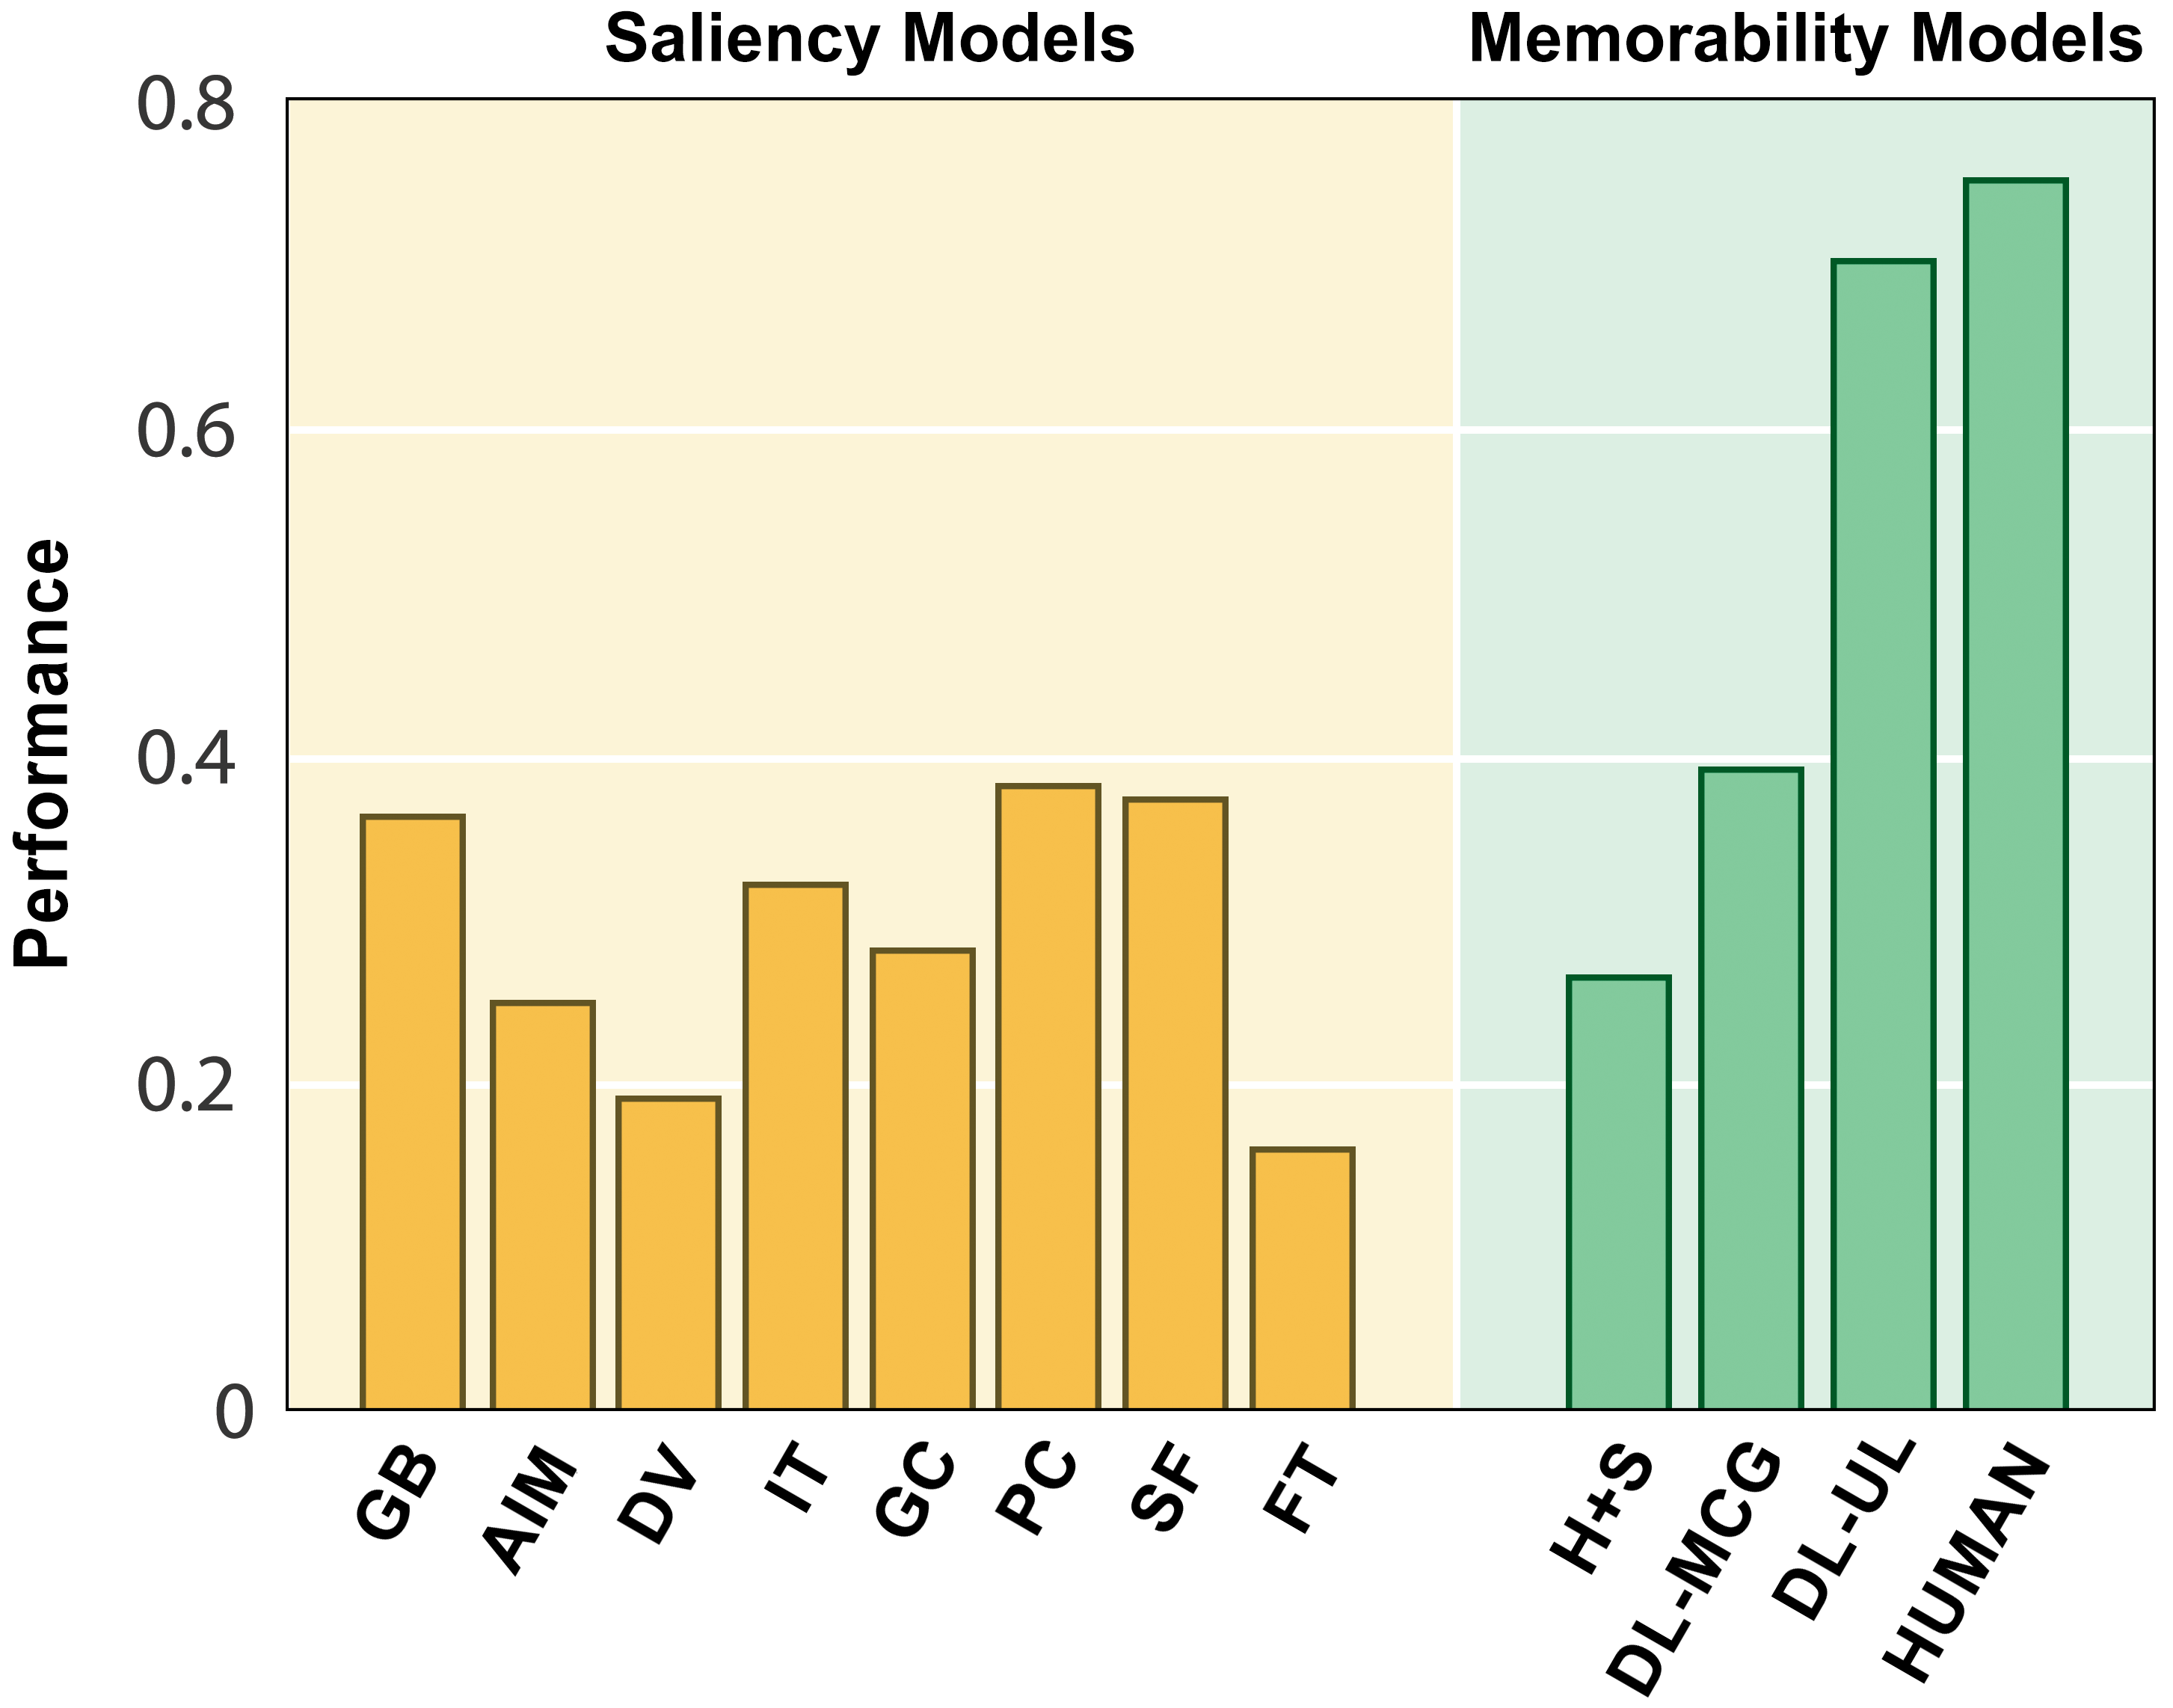
\includegraphics[width=0.5\textwidth]{figures/results/benchmark/comparison.png}}
\vspace{-5mm}\caption{\footnotesize\textbf{Main task.} add-in later. \B{put names of methods inside bars for brevity; replace performance with }}\label{fig:benchmark}
\end{figure}
